\documentclass[a4paper]{article}

\usepackage[utf8]{inputenc}
\usepackage[portuges]{babel}
\usepackage{indentfirst}
\usepackage{graphicx}

\title{Projeto de Laboratórios de Informática 3\\Grupo 21}
\author{Diogo Braga A82547 \and João Silva A82005 \and Ricardo Caçador A81064}
\date{\today}

\begin{document}

\maketitle

\begin{abstract}
  Este documento apresenta o projeto de Laboratórios de Informática
  3 (LI3), do curso de Engenharia Informática da Universidade
  do Minho.

  O projeto baseia-se na criação de um sistema de análise de ficheiros 
  XML que possuem informações do Stack Overflow, um website de perguntas
  e respostas sobre programação de computadores.

\end{abstract}

\tableofcontents
\listoffigures

\section{Introdução}
\label{sec:intro}

////////////////////// POR FAZER //////////////////////

Este documento apresenta uma possível estrutura para o relatório da 2ª
fase do projeto da disciplina de Laboratórios de Informática 1 (LI1),
da Licenciatura em Engenharia Informática da Universidade do Minho,
que toma a forma de um projeto de média dimensão a ser desenvolvido na
linguagem de programação funcional Haskell.

Nesse contexto, este relatório deve relatar o trabalho desenvolvido
pelos alunos para atingir o resultado final nesse projeto, devendo
acompanhar a submissão da solução implementada. Além de servir de
treino das capacidades de comunicação escrita dos estudantes, servirá
também como elemento de avaliação para a utilização de \LaTeX{} pelos
alunos. Sendo assim o código fonte \LaTeX{} do relatório deve ser
mantido no repositório \texttt{svn} atribuído ao grupo. Um relatório desta
natureza tem geralmente uma dimensão entre 4 e 8 páginas, para além de
eventuais anexos.

A \emph{introdução} de um relatório apresenta de modo geral o trabalho
descrito no relatório: o problema que se pretende resolver, a sua
contextualização e a abordagem proposta pelos alunos para o
resolver. Deve passar ao leitor não só uma perspetiva geral do
trabalho desenvolvido mas também a motivação por trás dele.

Esta secção termina normalmente com uma apresentação da estrutura do
relatório, sendo aqui apresentada uma sugestão. Neste caso, a Secção
~\ref{sec:estruturas} apresenta as estruturas de dados utilizadas 
no projeto, a Secção~\ref{sec:estrategias} indica as estratégias usadas 
para resolver as  questões apresentadas. O relatório termina com conclusões na
Secção~\ref{sec:conclusao}, onde é também apresentada uma análise
crítica dos resultados obtidos.Secção~\ref{sec:modularizacao}.

\section{Estruturas de Dados}
\label{sec:estruturas}

////////////////////// POR FAZER //////////////////////

////////////////////// TCD e TAD (ver aviso BB) //////////////////////

Esta secção tem as \emph{estruturas} do projeto.

\subsection{Estrutura TCD}
\begin{figure}[ht]
\centering
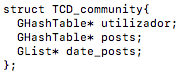
\includegraphics[scale=0.50]{image_tcd}
\caption{Estrutura TCD} 
\label{img:tcd}
\end{figure}

\subsection{Estrutura Utilizador}
\begin{figure}[ht]
\centering
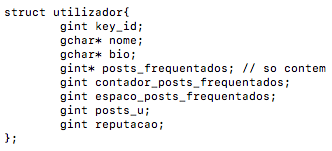
\includegraphics[scale=0.50]{image_utilizador}
\caption{Estrutura Utilizador} 
\label{img:utilizador}
\end{figure}

\subsection{Estrutura Posts}
\begin{figure}[ht]
\centering
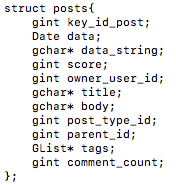
\includegraphics[scale=0.50]{image_posts}
\caption{Estrutura Posts} 
\label{img:posts}
\end{figure}

\section{Modularização}
\label{sec:modularizacao}

////////////////////// POR FAZER //////////////////////

\section{Estratégias das Interrogações}
\label{sec:estrategias}

\subsection{Init}

Função que cria a \textbf{TAD\_community}. Por consequência, inicializa
as estruturas relacionadas à struct \textbf{TCD\_community}, alocando
memória e usando a função da \textit{glib}, \textbf{g\_hash\_table\_new}.

\subsection{Load}

\subsection{Query 1}

Dado o identificador de um post, a função retorna o título do post 
e o nome de utilizador do autor. Se o post for uma resposta, a função
retorna o título e o id do utilizador da pergunta correspondente.

Nesta questão, sendo o valor do \textbf{id} igual ao da \textbf{key} 
da tabela de hash, recorremos à função da \textit{glib},
\textbf{g\_hash\_table\_lookup} que dado uma \textbf{key},
retorna o \textbf{value} associado. Caso nada seja encontrado,
é retornado NULL.

Tendo agora todos os valores referentes ao \textbf{post}, caso este
seja uma pergunta, é atríbuido à primeira coordenada o \textbf{title}
do post e à segunda o \textbf{nome} de quem realizou a questão.
Encontramos o \textbf{nome} do autor da questão invocando o parâmetro
\textbf{owner\_user\_id} na mesma função \textbf{lookup} utilizada 
anteriormente, passando agora a ser esse o \textbf{key/id} associado.

Caso seja uma resposta, o primeiro parâmetro é calculado usando a mesma 
função \textbf{g\_hash\_table\_lookup}, mas agora com o 
parâmetro \textbf{parent\_id}, que numa resposta retorna o \textbf{id} 
da pergunta ao qual esta respondeu. O segundo parâmetro é igualmente
calculado como se fosse uma pergunta, mudando apenas o novo 
\textbf{value} associado.

\subsection{Query 2}

Pretendemos obter o top N utilizadores com maior número de posts de 
sempre. Para isto, são considerados tanto perguntas quanto respostas 
dadas pelo respectivo utilizador.

////////////////////// POR FAZER //////////////////////

Nesta questão, utilizamos uma \textit{\textbf{GList*}} para armazenar 
os \textbf{values} de cada \textbf{utilizador}, sendo isto realizado
pela função da \textit{glib}, \textbf{g\_hash\_table\_get\_values}.

De seguida, percorremos a \textbf{lista} referida, e em cada posição
acedemos ao parâmetro \textbf{posts\_u}, que referencia o número de 
posts do utilizador em questão. Enquanto isso, fazemos a filtração
para o \textbf{set\_list}, tendo em conta se o utilizador que estamos
no momento atual possui mais \textbf{posts totais} que os \textbf{N} 
utilizadores que se encontram no set. Caso se conclua tal facto,
colocamos o seu \textbf{id} na posição estabelecida.

\subsection{Query 3}

Dado um intervalo de tempo arbitrário, obtemos o número total de posts 
(identificando perguntas e respostas separadamente) neste período.

Nesta questão, utilizamos uma \textit{\textbf{GList*}} para armazenar 
os \textbf{posts} ordenados por data que se encontram na estrutura 
\textbf{date\_posts}, para de seguida percorrer estes mesmos posts.

Enquanto isso, verificamos se a \textbf{data} do post se encontra entre 
os limites referenciados pela query, através da função \textbf{difDatas},
e caso seja uma pergunta, é incrementada a primeira coordenada do par,
caso contrário é uma resposta, e é incrementada a segunda coordenada.

\subsection{Query 4}

\subsection{Query 5}

Dado um ID de utilizador, devolvemos a informação do seu perfil (short 
bio) e os IDs dos seus 10 últimos posts (perguntas ou respostas), 
ordenados por cronologia inversa.

Nesta questão, recorremos à função da \textit{glib}, \textbf{g\_hash\_
table\_lookup}, para termos o \textbf{value} associado ao \textbf{id}
do utilizador. Desta forma, retornamos a \textbf{bio} do utilizador.

Retornamos os últimos 10 posts acedendo à estrutura que tem os posts
ordenados por data e, começando no último elemento da \textit{
\textbf{GList*}}, vamos percorrendo a lista para trás. Caso o \textbf{
owner\_user\_id} seja o requerido adicionamos o \textbf{id} do post à 
lista a retornar.

\subsection{Query 6}

Dado um intervalo de tempo arbitrário, devolver os IDs das N respostas 
com mais votos, em ordem decrescente do número de votos.

Nesta questão, recorremos à estrutura \textbf{date\_posts} que possuí 
as datas ordenadas. Caso o \textbf{post} seja uma pergunta e
se encontre entre as datas requeridas na query, é inserida numa nova
\textit{\textbf{GList*}} \textbf{glvotes} criada para armazenar os 
valores necessários para a resposta final.

Depois esta lista é ordenada por votos em ordem decrescente através da 
função da \textit{glib}, \textbf{g\_list\_sort}, que usa uma função de 
comparação \textbf{compara\_votes}, que tem em conta o \textbf{dif\_votes}
da estrutura. Finalmente acedemos ao \textbf{id\_post} relacionado, 
através dos dados respetivos da lista \textbf{glvotes}.

\subsection{Query 7}

Dado um intervalo de tempo arbitrário, devolver os IDs das N perguntas 
com mais respostas, em ordem decrescente do número de votos.

Nesta questão, recorremos à estrutura \textbf{date\_posts} que possuí 
as datas ordenadas. Caso o \textbf{post} seja uma pergunta e
se encontre entre as datas requeridas na query, é inserida numa nova
\textit{\textbf{GList*}} \textbf{glanswers} criada para armazenar os 
valores necessários para a resposta final.

Depois esta lista é ordenada por número de respostas em ordem decrescente 
através da função da \textit{glib}, \textbf{g\_list\_sort}, que usa uma 
função de comparação \textbf{compara\_answers}, que tem em conta o \textbf
{answer\_count} da estrutura. Finalmente acedemos ao \textbf{id\_post} 
relacionado, através dos dados respetivos da lista \textbf{glanswers}.

\subsection{Query 8}

\subsection{Query 9}

\subsection{Query 10}

\subsection{Query 11}

\subsection{Clean}

\section{Conclusões}
\label{sec:conclusao}

////////////////////// POR FAZER //////////////////////

A secção de \emph{conclusões} resume o restante documento, devendo
também apresentar uma análise crítica dos resultados atingidos tendo
em conta os objetivos definidos.

\end{document}